\documentclass{article}
\usepackage{tikz}
\usepackage{xcolor}

\definecolor{myblue}{RGB}{30,50,65}
\definecolor{bggray}{RGB}{240,240,240}

\begin{document}

\begin{center}
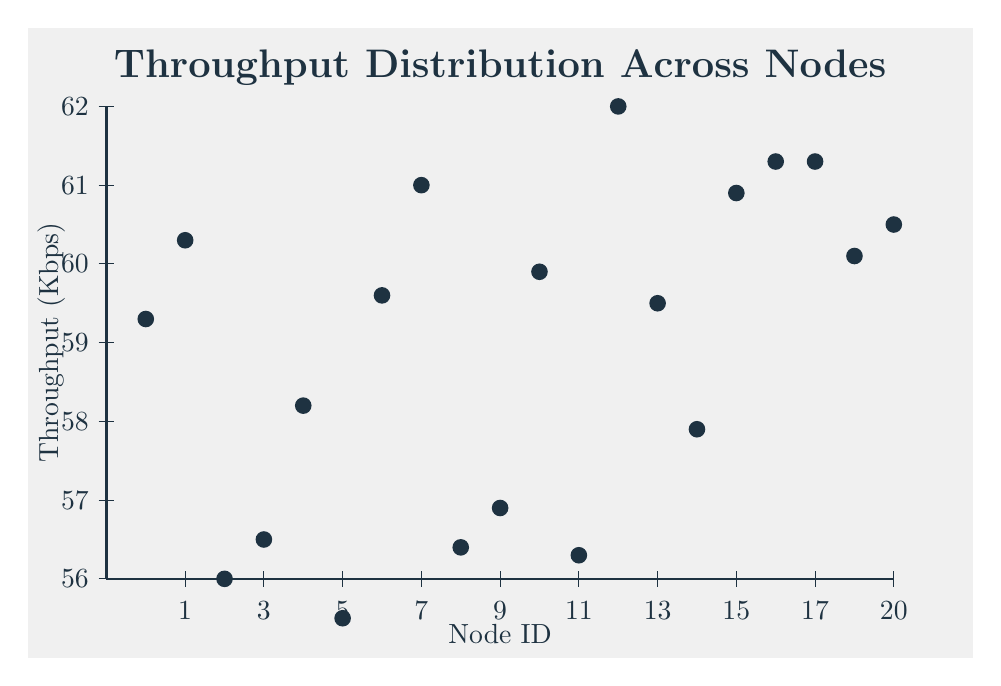
\begin{tikzpicture}

% Background
\fill[bggray] (0,0) rectangle (12,8);

% Axes
\draw[thick, myblue] (1,1) -- (1,7); % Y-axis
\draw[thick, myblue] (1,1) -- (11,1); % X-axis

% Title
\node[text=myblue, font=\Large\bfseries] at (6,7.5) {Throughput Distribution Across Nodes};

% Labels
\node[text=myblue] at (6,0.3) {Node ID};
\node[rotate=90, text=myblue] at (0.3,4) {Throughput (Kbps)};

% Y-axis ticks (56–62)
\foreach \y/\val in {1/56,2/57,3/58,4/59,5/60,6/61,7/62} {
    \draw[myblue] (0.9,\y) -- (1.1,\y);
    \node[left, text=myblue] at (0.9,\y) {\val};
}

% X-axis ticks (1–20)
\foreach \x in {2,3,4,5,6,7,8,9,10,11} {
    \draw[myblue] (\x,0.9) -- (\x,1.1);
}
\foreach \x/\val in {
2/1,3/3,4/5,5/7,6/9,7/11,8/13,9/15,10/17,11/20
} {
    \node[text=myblue] at (\x,0.6) {\val};
}

% Scaling (56–62 → 1–7)
\def\scale{1}

% Data points
\foreach \x/\y in {
1/59.3,2/60.3,3/56.0,4/56.5,5/58.2,
6/55.5,7/59.6,8/61.0,9/56.4,10/56.9,
11/59.9,12/56.3,13/62.0,14/59.5,15/57.9,
16/60.9,17/61.3,18/61.3,19/60.1,20/60.5
} {
    \fill[myblue] ({1 + \x*0.5},{1 + (\y-56)*\scale}) circle (3pt);
}

\end{tikzpicture}
\end{center}

\end{document}